% Figure: the ladder of local media, the maximum-principle cut, and the homogeneous
% slice. Referenced from §10's opener. Pure TikZ; new design (plan table: "ladder with
% cut and slice").
%
% Pedagogic point: order n is a rung; rung n is an (n-1)-parameter family of admissible
% local media (prop:local-ladder); the PMP cuts between n = 2 and n = 3 (thm:locality);
% the homogeneous members a_j = j/n are one point per rung, the α = 1/n stable cases of
% 2005 (rem:stable-slice) — so the 2005 point α = ½ is where the slice meets the cut.

\begin{figure}[t]
\centering
\begin{tikzpicture}[every node/.style={font=\small}, line cap=round, >=stealth]

% rungs: order n at height 1.5n
\foreach \n/\y/\len/\lab in {1/1.5/1.2/{$n=1$: transport $-c'\partial_x$ (degenerate)},
                             2/3.0/4.4/{$n=2$: the Bessel line, one parameter $a$},
                             3/4.5/5.6/{$n=3$: two parameters $a_1, a_2$},
                             4/6.0/6.4/{$n=4$: three parameters}} {
  \draw[very thick] (0,\y) -- (\len,\y);
  \node[anchor=west] at (6.7,\y) {\lab};
}
\node[anchor=west] at (0.0,6.9) {$\vdots$\quad every order $n$: an $(n-1)$-parameter rung (Proposition~\ref{prop:local-ladder})};

% the PMP cut between n=2 and n=3
\draw[dashed, thick] (-0.4,3.75) -- (10.6,3.75);
\node[anchor=west] at (0.0,4.05) {positive maximum principle: only $n \le 2$ survive (Theorem~\ref{thm:locality})};

% the homogeneous slice: one point per rung at a_j = j/n
\draw[gray, thick] plot[smooth] coordinates {(0.9,1.5) (2.1,3.0) (2.9,4.5) (3.4,6.0)};
\foreach \x/\y in {0.9/1.5, 2.1/3.0, 2.9/4.5, 3.4/6.0} \fill (\x,\y) circle (1.7pt);
\node[gray!40!black, anchor=south west] at (3.5,6.05) {homogeneous slice: $\alpha = 1/n$};

% the 2005 point
\node[anchor=north west] at (2.2,2.9) {$\alpha = \tfrac12$, $a = \tfrac12$: the heat-signaling member};

\end{tikzpicture}
\caption{The ladder of local media. Locality alone admits media of every order: rung $n$ is
the $(n-1)$-parameter family of Proposition~\ref{prop:local-ladder}, with $n = 1$ the
degenerate transport member. The positive maximum principle cuts the ladder between orders
two and three (Theorem~\ref{thm:locality}), leaving the transport member and the Bessel
line. The homogeneous (semigroup) members are one point per rung, the stable cases
$\alpha = 1/n$ of \sscite{fagerstrom2005temporal} (Remark~\ref{rem:stable-slice}); the
maximum principle acts on them the same way, and what survives of the slice is the single
point $\alpha = \tfrac12$ --- the heat-signaling equation --- which under the hemigroup
axioms unfolds into the full Bessel rung.}
\label{fig:ladder}
\end{figure}
